\section{Introduction}

Phenology, the timing of seasonal biological phenomena, is a key aspect of plant and animal life.
It defines the timing and duration of growth and reproduction and thereby determines the ability to capture seasonally variable resources.
The study of plant and animal phenology has allowed for a better understanding of fundamental ecosystem processes such as biogeochemical cycles,
trophic interactions, animal migrations, and the response of populations and communities to global climate change,
as well as informing applications in agriculture, forestry, and public health such as varietal selection in plant and animal breeding, or integrated pest and disease management \citep{chuine2017process}.

Phenological analyses often focus on the timing of events, such as the dates of plant flowering \citep{aono2008phenological}.%, the dates of egg laying in birds \cite{shutt2019environmental}, or the dates of first or peak appearance of butterflies \citep{roy2000phenology}.
However, for many biological phenomena exact dates of particular events are more difficult to observe than the state of the system itself.
For example, repeated but sparse survey visits may enable the recording of whether a plant is in bud, flowering, or setting fruit, but not the exact dates when each of those stages was reached.
%Similarly, surveys may record the development stage of insects or amphibians, or the breeding or moult status of birds.
Such observations can be used to categorize an organism's state into discrete classes.
Further, as the progression of the annual cycle often results in a natural ordering of these classes, e.g. from least to most developed, the resulting data can be described using ordinal regression models \cite{mccullagh1980regression,agresti2010analysis}.

I here replicate a number of ordinal regression models that were developed by \citet{dennis1986stochastic} and \citet{candy1991modeling} to describe insect phenology. 

\section{Data}
The models replicated in this study are fitted to a data set on the phenology of the western spruce budworm \emph{Choristoneura freemani} (Lepidoptera: Tortricidae), a defoliating moth that is widespread in western North America \citep{brookes1987western}. This data set was originally published in \citep{dennis1986stochastic} and is a subset of a larger budworm survey data set analysed in \citep{kemp1986}. The data consist of 12 sampling occassions at which counts of individual budworms in each of seven development stages (five larval instars, pupae, and adults) were recorded. The only available covariate is a measure of seasonal progression, the accumulated degree days calculated using a threshold of 5.5°C. \citet{candy1991modeling} noted an inconsistency in these data, namely that the reported total number of individuals did not correspond to the sum across the seven development stages for two of the sampling occasions. I therefore use the data set as it was republished in \citet{candy1990biology}, where numbers in each stage have been assumed correct and the totals for each sampling occasion were adjusted accordingly.

\section{Methods}
The statistical models replicated here are different types of ordinal regression models \citep{agresti} all with the aim of predicting the proportion of an insect population in a particular development stage at any given given time. In particular, they represent three different parametrisations of the so-called cumulative model and one version of the so-called continuation ratio model \citep{}. A recent summary of the theory underlying these models is provided in \citep{buerkner?}.


models presented are  \citet{dennis1986stochastic} and \citet{candy1991modeling} 

The models generally assume that the development of an insect follows an unobservable stochastic process $S(t)$ consisting of accumulated increments of development over time $t$. As the amount of $S(t)$ increases, the insect passes through successive stages, delimited by moults, with the $j$th moult occuring when the development threshold $a_j$ is reached:

\begin{alignat*}{3}
  \mathrm{stage}\,1&:\qquad {}&   S(t) & \leq a_1 \\
  \mathrm{stage}\,2&:\qquad  a_1&< S(t) & \leq a_2 \\
  \vdots & &\vdots \\
  \mathrm{stage}\,r-1&:\qquad  a_{r-2}&< S(t) & \leq a_{r-1} \\
  \mathrm{stage}\,r&:\qquad  a_{r-1}&< S(t) 
\end{alignat*}

The $a_j$ values are typically unknown and must be estimated from the data.

\subsection{Ordinal regression model with constant variance }
If the cumulative number of individuals observed in stages 1 to $j$ is given by $m_{ij}=\sum_{k=1}^jn_{ik}$ then the ordinal regression model \citep{mccullagh1980} is specified by %TODO: tidy up indices r vs j to be consistent in enumerating the stages
\begin{alignat}{1}
\mathbf{E}(m_{ij})&=N_iPr(S(t) < \alpha_j), \qquad j = 1,\dots ,r\\
&=N_iG(\alpha_j + \beta z_i)
\end{alignat}
where $G$ is the cumulative probability density function of $S(t)$, $\alpha_j$ are ordered thresholds or cut-point parameters, $\beta$ is a vector of regression parameters and $z_i$ is a vector of predictor variables.
If the probability of an individual being in stage $j$ or earlier at time $t_i$ is $$\mu_{ij} = \mathbf{E}(m_{ij})/N_i$$ one can define $G^{-1}$ as the link function of a generalised linear model with the linear predictor $$\eta_{ij}=\alpha+\beta z_i$$. This ordinal regression model is commonly known as the cumulative model, and is applied to the budworm data in \citep{candy1991modeling} using the logit and complementary log-log link functions. In  both cases the parametrisation results in a constant variance for $S(t)$. \citet{candy1991modeling} reexpresses the model in terms of stage-specific counts $n_{ij}$  
\begin{equation}
\mathbf{E}(n_{ij})=N_i\{G(\alpha_j + \beta z_i) - G(\alpha_{j-1} + \beta z_i)\}
\end{equation}
and fits it using a Poisson likelihood \citep{thompson1981composite}. The original paper provides a set of example macros for the software package \verb+GLIM+ \citep{aitkin1989statistical} which is no longer actively developed or distributed. However, the cumulative model is implemented in various R packages, including \verb+VGAM+ \citep{VGAM} and \verb+ordinal+ \cite{ordinal} and I here make use of these to fit the model to the budworm data.
\subsection{Ordinal regression model with proportional variance}
\citet{dennis1986stochastic} proposed a different parametrisation of the ordinal model is based on assuming a logistic distribution for $S(t)$, such that the probability that an insect's development at time $t$ has not exceeded $s$ amounts to 
\begin{equation}
Pr[S(t) \leq s] = 1 \bigg/ \left\{ 1 + \exp\left[-\left(\frac{s-t}{\sqrt{b^2t}}\right)\right]\right\}
\end{equation}
where $b^2$ is a positive constant which also must be estimated from the data. This distribution has a mean of $t$ and a variance of $(\pi^2/3)b^2t$.
At any fixed time $t$ the thresholds $a_j$ segment the porbaility distribution function in to $r$ parts and the area under the curve between $a_{i-1}$ and $a_i$ gives the probability that the insect will be in stage $i$ at time $t$.

This modelling approach is applied to a dataset consisting of samples that record the number of insects $x_{ij}$ in stage $j$ at times $t_1, t_2, \dots, t_q$ and the $x_{ij}$ are assumed to be random samples from a multinomial distribution with corresponding multinomial probabilities $p_{ij}$

\begin{align}
p_{ij} & = Pr[a_{j-1} < S(t_i) \leq a_{j}]\\
& = 1 \bigg/ \left\{ 1 + \exp\left[-\left(\frac{a_j-t_i}{\sqrt{b^2t_i}}\right)\right]\right\} - 1 \bigg/ \left\{ 1 + \exp\left[-\left(\frac{a_{j-1}-t_i}{\sqrt{b^2t_i}}\right)\right]\right\}
\end{align}

To fulfill the constraint that $\sum_{j=1}^r p_{ij}= 1$ it is further assumed that $a_0 = -\infty$ and $a_r = +\infty$.
The model has $r$ unknown parameters $a_1, \dots, a_{r-1}$ and $b^2$ which can be found by maximising the corresponding log-likelihood function which takes the form 
\begin{equation}
\mathcal{\ell} = \log C + \sum_{j=1}^r \sum_{i=1}^q x_{ij} \log p_{ij}
\label{eq:dennis_loglik}
\end{equation}
where $C$ is a combinatorial constant that is independent of the parameter values.

\citet{dennis1986stochastic} provided SAS code to estimate the parameters under this likelihood using an interatively reweighted non-linear least squares approach based on \verb+PROC NLIN+. This code only required minimal updates to run in a contemporary version of SAS (SAS 9.4) and is provided in the article repository. However, since SAS is a proprietary software package, I created an R version of the estimation procedure which directly optimizes the log-likelihood (\ref{eq:dennis_loglik}) using the \verb+optim+ function and initial values provided in \citep{dennis1986stochastic}.

\citet{dennis1986stochastic}

\subsection{Continuation ratio model}

\section{Results}
\begin{figure}[p]
  \centering
  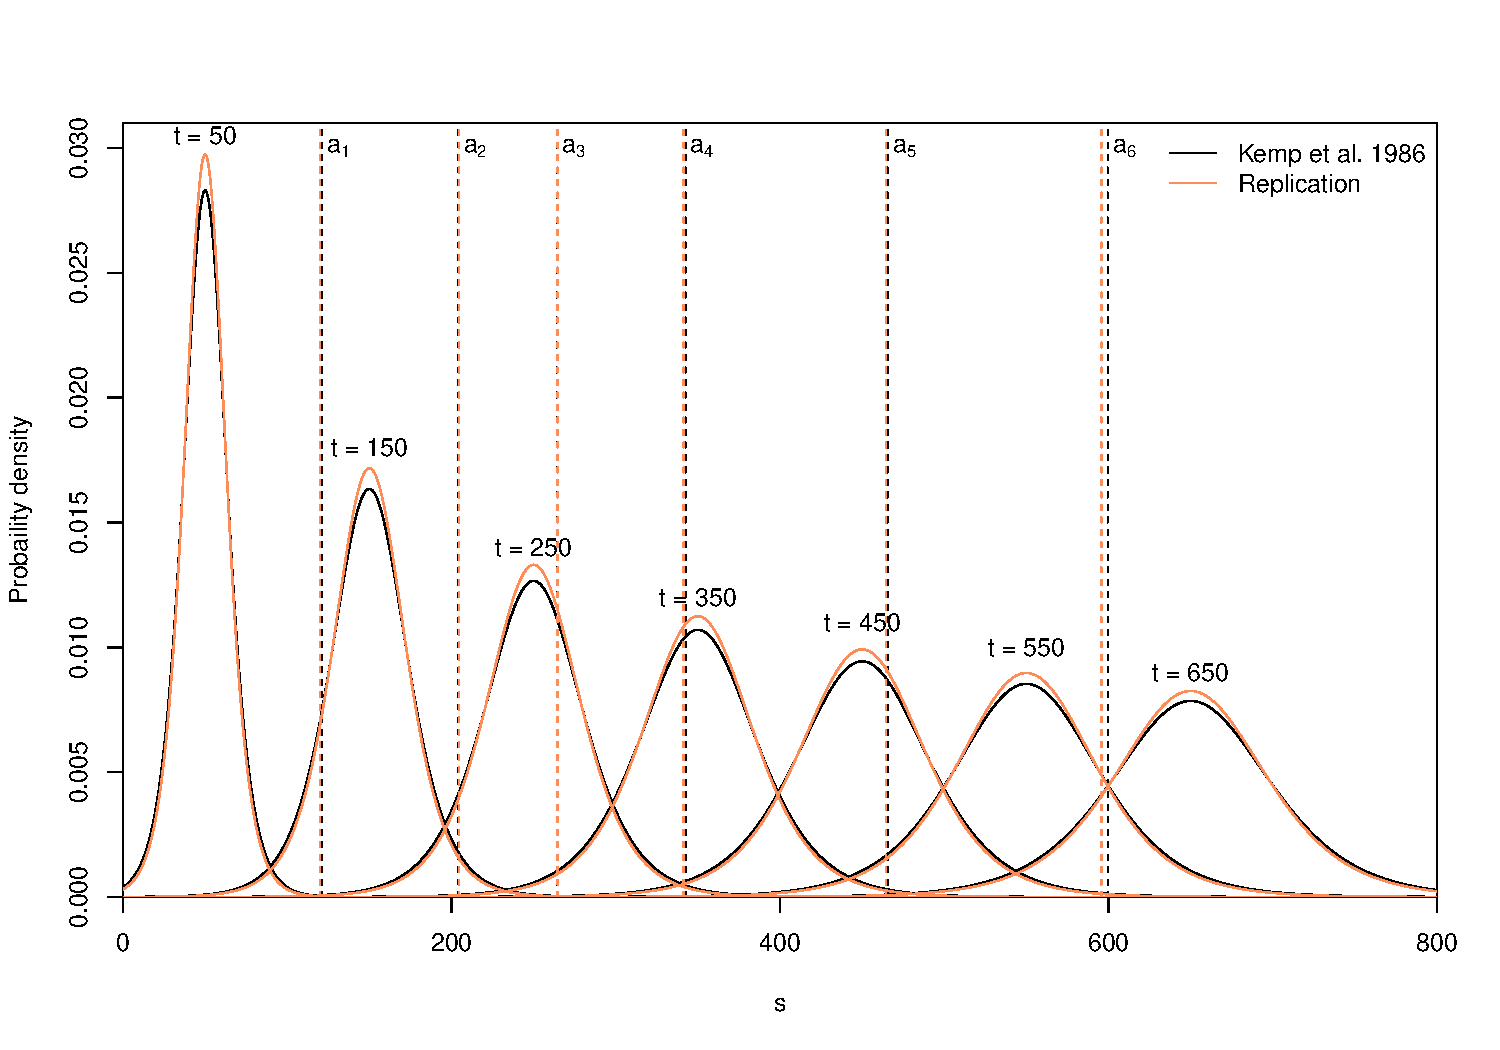
\includegraphics[width=\textwidth]{../figures/dennis_fig2.pdf}
  \caption{Logistic PDF of the \citet{dennis1986stochastic} model plotted for seven fixed values of~$t$. Area under the PDF between $a_{j-1}$ and $a_j$ gives the expected proportion of insects in stage $j$ at time $t$. Values of $a_j$ and $b^2$ used in the graph are the estimates given in Table 1 of \citep{kemp1986stochastic} (black lines) and the estimates from the replication (red lines). This figure replicates Figure 2 in \citep{dennis1986stochastic}.}
  \label{fig:fig1}
\end{figure}

\section{Results}
\begin{figure}[p]
  \centering
  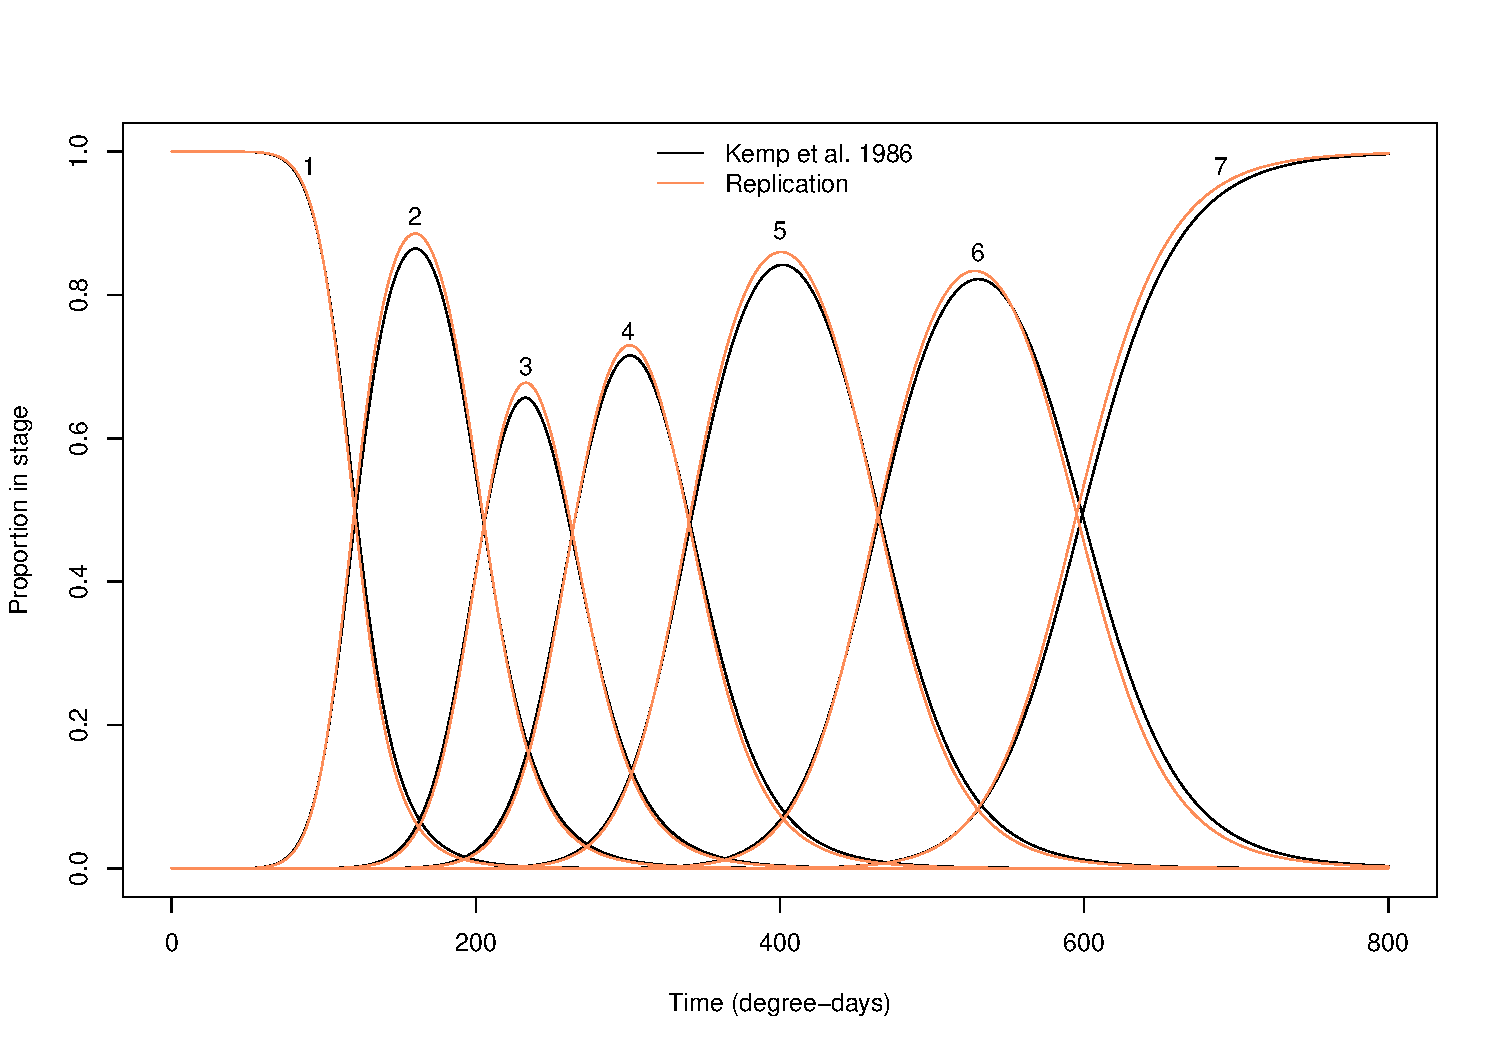
\includegraphics[width=\textwidth]{../figures/dennis_fig3.pdf}
  \caption{Expected proportion of insects in stages 1-7 plotted as functions of time $t$. Values of $a_j$ and $b^2$ used in the graph are the estimates given in Table 1 of \citep{kemp1986stochastic} (black lines) and the estimates from the replication (red lines). This figure replicates Figure 3 in \citep{dennis1986stochastic}.}
  \label{fig:fig2}
\end{figure}